\begin{frame}{Exemplo de {\it hash} perfeito}

    \begin{figure}
        \centering
        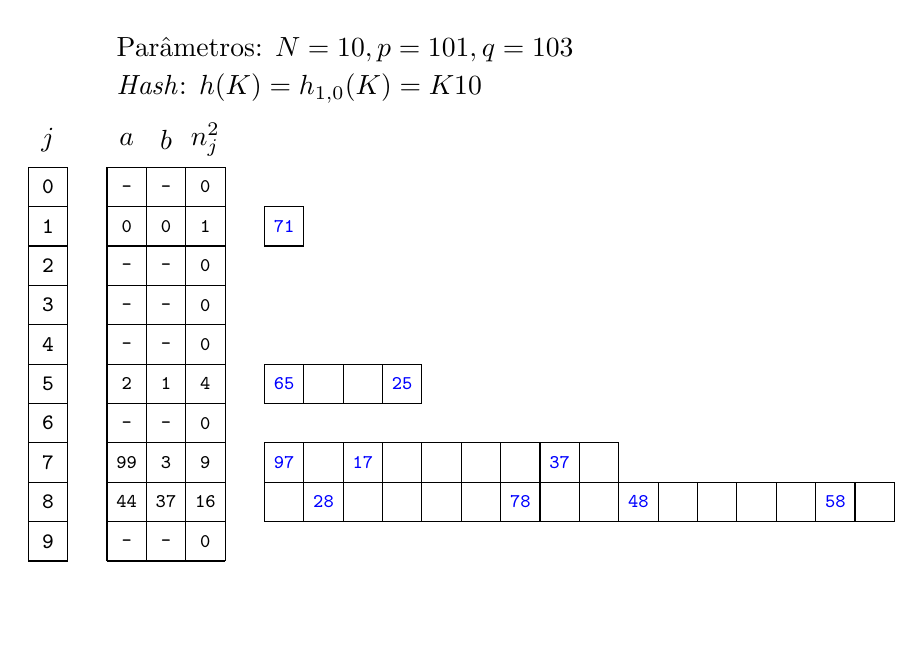
\begin{tikzpicture}
            \node[anchor=west] at (1, 6.5) { Parâmetros: $N = 10, p = 101, q = 103$ };
            \node[anchor=west] at (1, 6) { \textit{Hash}: $h(K) = h_{1,0}(K) = \Mod{K}{10}$ };

            \begin{scope}[scale=0.5]
                \node at (0.5, 10.7) { $j$ };
                \node at (2.5, 10.7) { $a$ };
                \node at (3.5, 10.7) { $b$ };
                \node at (4.5, 10.7) { $n_j^2$ };

                \node at (0.5, 9.5) { \footnotesize \tt \textbf{0} };
                \node at (0.5, 8.5) { \footnotesize \tt \textbf{1} };
                \node at (0.5, 7.5) { \footnotesize \tt \textbf{2} };
                \node at (0.5, 6.5) { \footnotesize \tt \textbf{3} };
                \node at (0.5, 5.5) { \footnotesize \tt \textbf{4} };
                \node at (0.5, 4.5) { \footnotesize \tt \textbf{5} };
                \node at (0.5, 3.5) { \footnotesize \tt \textbf{6} };
                \node at (0.5, 2.5) { \footnotesize \tt \textbf{7} };
                \node at (0.5, 1.5) { \footnotesize \tt \textbf{8} };
                \node at (0.5, 0.5) { \footnotesize \tt \textbf{9} };

                \node at (2.5, 9.5) { \scriptsize \tt - };
                \node at (3.5, 9.5) { \scriptsize \tt - };
                \node at (4.5, 9.5) { \scriptsize \tt 0 };

                \node at (2.5, 8.5) { \scriptsize \tt 0 };
                \node at (3.5, 8.5) { \scriptsize \tt 0 };
                \node at (4.5, 8.5) { \scriptsize \tt 1 };
                \node at (6.5, 8.5) { \scriptsize \tt \textcolor{blue}{71} };

                \node at (2.5, 7.5) { \scriptsize \tt - };
                \node at (3.5, 7.5) { \scriptsize \tt - };
                \node at (4.5, 7.5) { \scriptsize \tt 0 };

                \node at (2.5, 6.5) { \scriptsize \tt - };
                \node at (3.5, 6.5) { \scriptsize \tt - };
                \node at (4.5, 6.5) { \scriptsize \tt 0 };

                \node at (2.5, 5.5) { \scriptsize \tt - };
                \node at (3.5, 5.5) { \scriptsize \tt - };
                \node at (4.5, 5.5) { \scriptsize \tt 0 };

                \node at (2.5, 4.5) { \scriptsize \tt 2 };
                \node at (3.5, 4.5) { \scriptsize \tt 1 };
                \node at (4.5, 4.5) { \scriptsize \tt 4 };
                \node at (6.5, 4.5) { \scriptsize \tt \textcolor{blue}{65} };
                \node at (9.5, 4.5) { \scriptsize \tt \textcolor{blue}{25} };

                \node at (2.5, 3.5) { \scriptsize \tt - };
                \node at (3.5, 3.5) { \scriptsize \tt - };
                \node at (4.5, 3.5) { \scriptsize \tt 0 };

                \node at (2.5, 2.5) { \scriptsize \tt 99 };
                \node at (3.5, 2.5) { \scriptsize \tt 3 };
                \node at (4.5, 2.5) { \scriptsize \tt 9 };
                \node at (8.5, 2.5) { \scriptsize \tt \textcolor{blue}{17} };
                \node at (13.5, 2.5) { \scriptsize \tt \textcolor{blue}{37} };
                \node at (6.5, 2.5) { \scriptsize \tt \textcolor{blue}{97} };

                \node at (2.5, 1.5) { \scriptsize \tt 44 };
                \node at (3.5, 1.5) { \scriptsize \tt 37 };
                \node at (4.5, 1.5) { \scriptsize \tt 16 };
                \node at (7.5, 1.5) { \scriptsize \tt \textcolor{blue}{28} };
                \node at (15.5, 1.5) { \scriptsize \tt \textcolor{blue}{48} };
                \node at (20.5, 1.5) { \scriptsize \tt \textcolor{blue}{58} };
                \node at (12.5, 1.5) { \scriptsize \tt \textcolor{blue}{78} };

                \node at (2.5, 0.5) { \scriptsize \tt - };
                \node at (3.5, 0.5) { \scriptsize \tt - };
                \node at (4.5, 0.5) { \scriptsize \tt 0 };

                \draw (0,0) grid (1, 10);
                \draw (2,0) grid (5, 10);
                \draw (6,8) grid (7, 9);
                \draw (6,4) grid (10, 5);
                \draw (6,2) grid (15, 3);
                \draw (6,1) grid (22, 2);

                \draw[white] (0, -2);
            \end{scope}

        \end{tikzpicture}
    \end{figure}

\end{frame}
